\vspace{-0.1in}
\section{Experimental Results} \label{sec:results}
\vspace{-0.1in}
In this section, we evaluate the performance of our bisection and twisted algorithm and compare it with prior SVD implementations on CPUs and GPUs.
%We also evaluate the performance of BT on huge matrices of size more than $100K$. 
%To our knowledge, this has not been done in any of the prior work so far. 
We implement the proposed BT algorithm on Tesla K40c with Kerpler architecture. 
Our implementation can run on GeForce 750Ti with Maxwell architecture and Quandro with Fermi architecture. 
%three different GPUs: GeForce 750 Ti, Quadro 600 and Tesla K40c,
%which differ in architecture, memory size and bandwidth listed in Table \ref{tab:spec}. 
In our implementations, we set the number of threads per GPU block as 512, which brings the better performance than other possible block sizes.
For the multi-GPU version of BT, we use 2 Tesla K40c that reside in the same server to scale up the size of matrices. 
%For the multi-GPU version of BT, we use a mixture of these GPUs that reside in the same server to scale up the size of matrices. 
%It is worth noting that our multi-GPU version of BT algorithm can be extended to physically distributed GPUs, i.e., GPUs on different hosts connected via a high speed network. 
%This part is however beyond the scope of this paper. 
%\begin{table}[h]
%\vspace{-0.2in}
%\caption{Specifications of Different GPUs}
%\vspace{-0.1in}
%\centering
%\begin{tabular}{|c|c|c|c|}
%\hline
%Specifications & GeForce 750 & Quandro 600 & Tesla K40 \\ \hline
%Architecture   &     Maxwell &       Fermi &    Kepler \\ \hline
%CUDA Cores     &         640 &          96 &      2880 \\ \hline
%TFLOPS         &       1.306 &       0.246 &      4.29 \\ \hline
%GPU Clock      &    1268 MHz &    1280 MHz &   745 MHz \\ \hline
%Mem Size       &        2 GB &        1 GB &     12 GB \\ \hline
%Mem Bandwidth  &   86.4 GB/s &   25.6 GB/s &  288 GB/s \\ \hline
%\end{tabular}
%\label{tab:spec}
%\vspace{-0.5in}
%\end{table}

\subsection{Comparison to Existing SVD Implementations}
We generate random bidiagonal matrices with double precision numbers in the range between 0 and 1.
In order to achieve high confidence on the results, we generate 10 random matrices, and for each matrix, our SVD algorithm is executed 10 times on a GPU (or two GPUs).
The standard deviation of their execution time is very small, so we report the average execution time across the 100 runs as the performance results.

We compare our algorithm with CULA GPU library \cite{cula}, Intel MKL library \cite{mkl}, Sheetal's QR implementation on S1070 \cite{09IPDPSQR}, and Liu's DC implementation on M2070 \cite{13CFDC}.
We measure the performance of CULA on Tesla K40c, and that of Intel MKL on an 8-core 2.53GHz CPU.
Until now, CULA library only has a QR based routine called culaDbdsqr.
Intel MKL library has both DC routine DBDSDC and QR routine DBDSQR. We select a faster routine DBDSDC for a comparison.
For Sheetal's \cite{09IPDPSQR} and Liu's \cite{13CFDC} implementation, we use the experimental results presendted in their paper. 

\begin{figure}[hbpt]
\vspace{-0.3in}
\centering
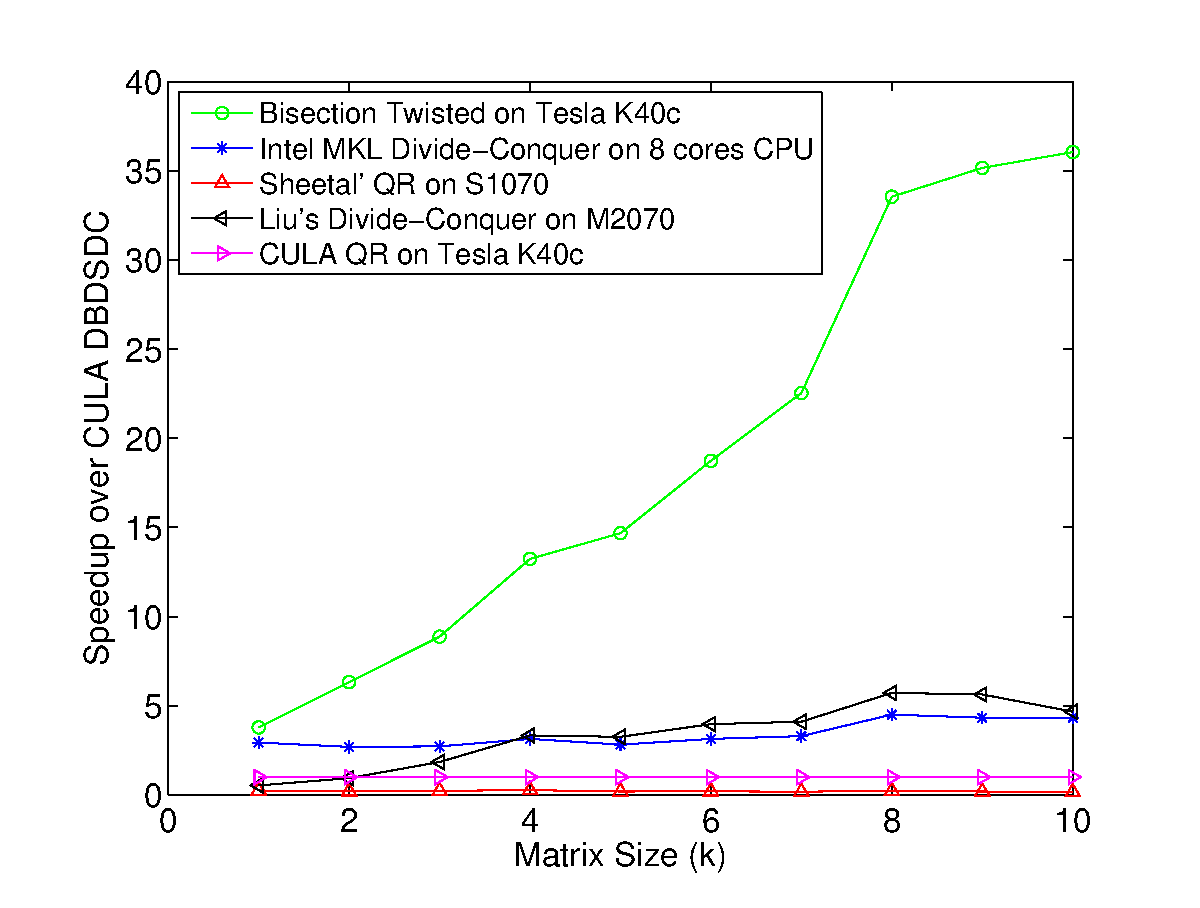
\includegraphics[width=0.5\textwidth,height=1in]{svd_speedup}
\vspace{-0.2in}
\caption{Overall Performance Comparison}
\label{fig:svd_speedup}
\vspace{-0.3in}
\end{figure}
Figure \ref{fig:svd_speedup} shows the performance comparison of BT
implementation on Tesla K40c GPU to other existing libraries
and implementations.
The x-axis is the size of input matrix, and the y-axis is the speedup
using CULA QR routine DBDSQR as the baseline.
Our BT algorithm achieves a speedup of 3.8 to 36 over CULA culaDbdsqr routine,
while Intel MKL DBDSDC routine has a 2.9 to 4.3 speedup on a 8 core CPU and Liu's implementation achieves only 0.5 to 4.7 speedup over CULA library.
On the other hand, Sheetal's implementation is about 3 to 5.3 times slower than CULA library.

The performance of BT scales well when the matrix size becomes large.
Overall, we achieve a speedup of 1.3 to 8.3 over the Intel MKL
DC implementation on CPU, 4 to 7.2 over the Liu's
DC method on GPU, and 15 to 288 over the QR implementation in the work by Sheetal et al.
Now let us take a look at each of the algorithms from the perspective of matrix size, Sheetal's QR implementation and Liu's DC implementation do not work at all when the dimensions of matrices are larger than 14K by 14K on their GPU with memory size of 16GB and 6GB, respectively. In contrast, in our implementation, the matrix size could reach 1 million by 1 million as shown in Table \ref{tab:hugeResultTesla}.

\if 0
\vspace{-0.2in}
\subsection{Performance Comparison on Different GPUs}

\subsubsection{Singular Value Computation}
\begin{figure}[hbpt]
\vspace{-0.3in}
\centering
  \subfigure[Execution time]
  {
    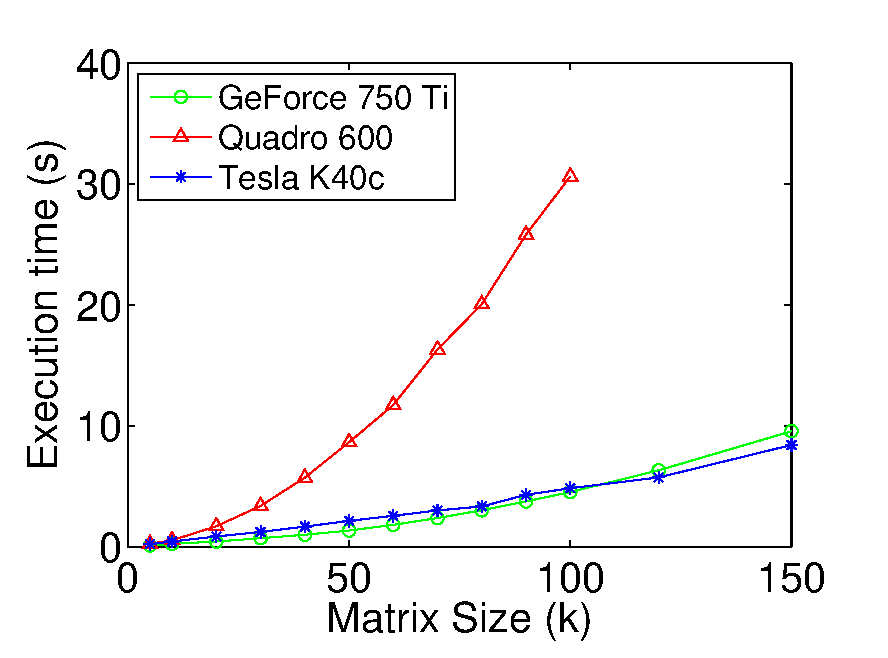
\includegraphics[width=0.3\textwidth,height=1in]{svd_val_gpus}
    \label{fig:svd_val}
  }
  \subfigure[Profiling Data]
  {
    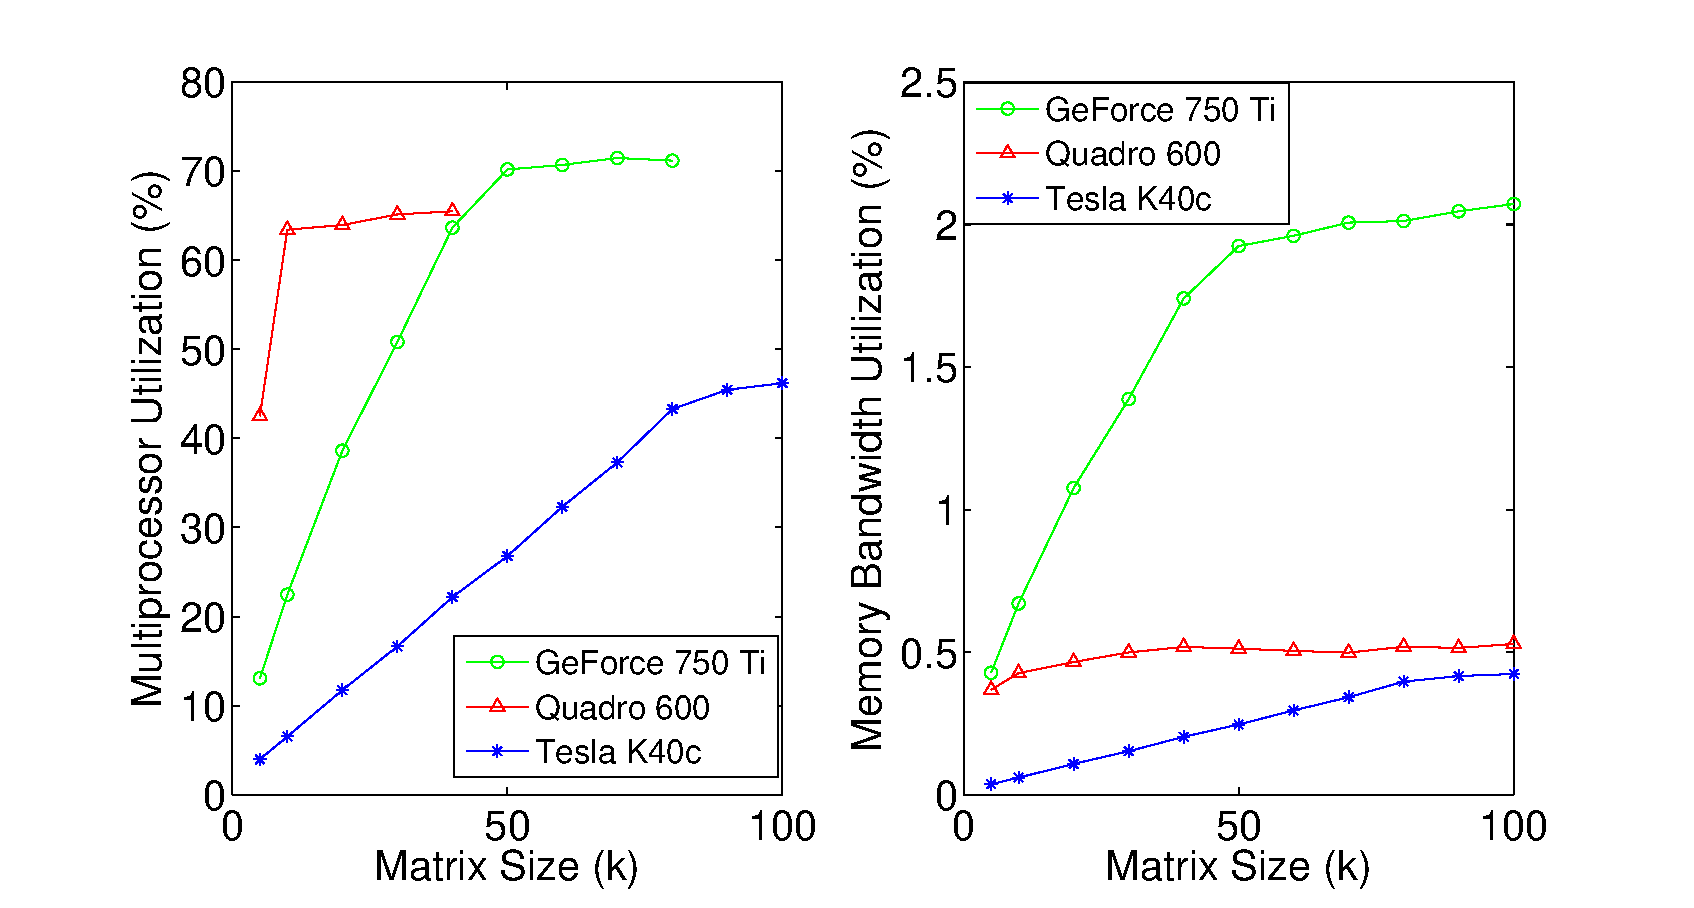
\includegraphics[width=0.6\textwidth,height=1in]{svd_val_gpus_prof}
    \label{fig:svd_val_prof}
  }
\vspace{-0.1in}
  \caption{Singular Value Kernel on Different GPUs}
  \label{fig:svdval}
\vspace{-0.3in}
\end{figure}

Figure \ref{fig:svd_val} shows the execution time of calculating singular values with our ``equal number division'' design on different GPUs with single-precision floating point.
Quadro has the worst performance, while performance of GeForce and Tesla are close to each other.
In particular, When the matrix size is less than $100K$, GeForce is slightly better. Otherwise, Tesla is better. 

To understand the reasons
of such performance differences, we conduct a series of profiling experiments.
Figure \ref{fig:svd_val_prof} shows the thread activity and memory bandwidth utilizations of singular value kernels on different GPUs, for matrices of size up to 
100K (unfortunately we are unable to get profiling data for matrices of larger size due to the overflow of profiling counters). 
The figure shows that the thread utilization reaches 70\% on Quadro and GeForce, and 50\% on Tesla. 
But the memory bandwidth utilization is only 0.1\%-2\%.
The main reason is that singular value computations rely on the fast shared memory
of GPUs due to its low memory requirements. That is, finding the singular
values is rather CPU-bound than memory-bound. 
As a result, the performance is determined largely by the number of CUDA cores and the ratio of thread activity on a GPU.

\subsubsection{Singular Vector Computation}
Figure \ref{fig:svd_vec} shows the execution time of singular vector kernel on different GPUs. 
It is easily seen that GeForce is about 8 times faster than
Quadro. This is because GeForce has a much higher memory bandwidth
than Quadro.
In addition, the device memory read/write transactions of GeForce are only 1/6 and 1/4 of those of Quadro, respectively.
The performance on Tesla is slightly better than that on GeForce.
Tesla has nearly the same device memory read transactions as GeForce does, while 3 times more write transactions than GeForce.
Yet Tesla is still the winner of the three because of its extremely high
bandwidth as listed in Table~\ref{tab:spec}.

\begin{figure}[hbpt]
\vspace{-0.3in}
\centering
  \subfigure[Execution time]
  {
    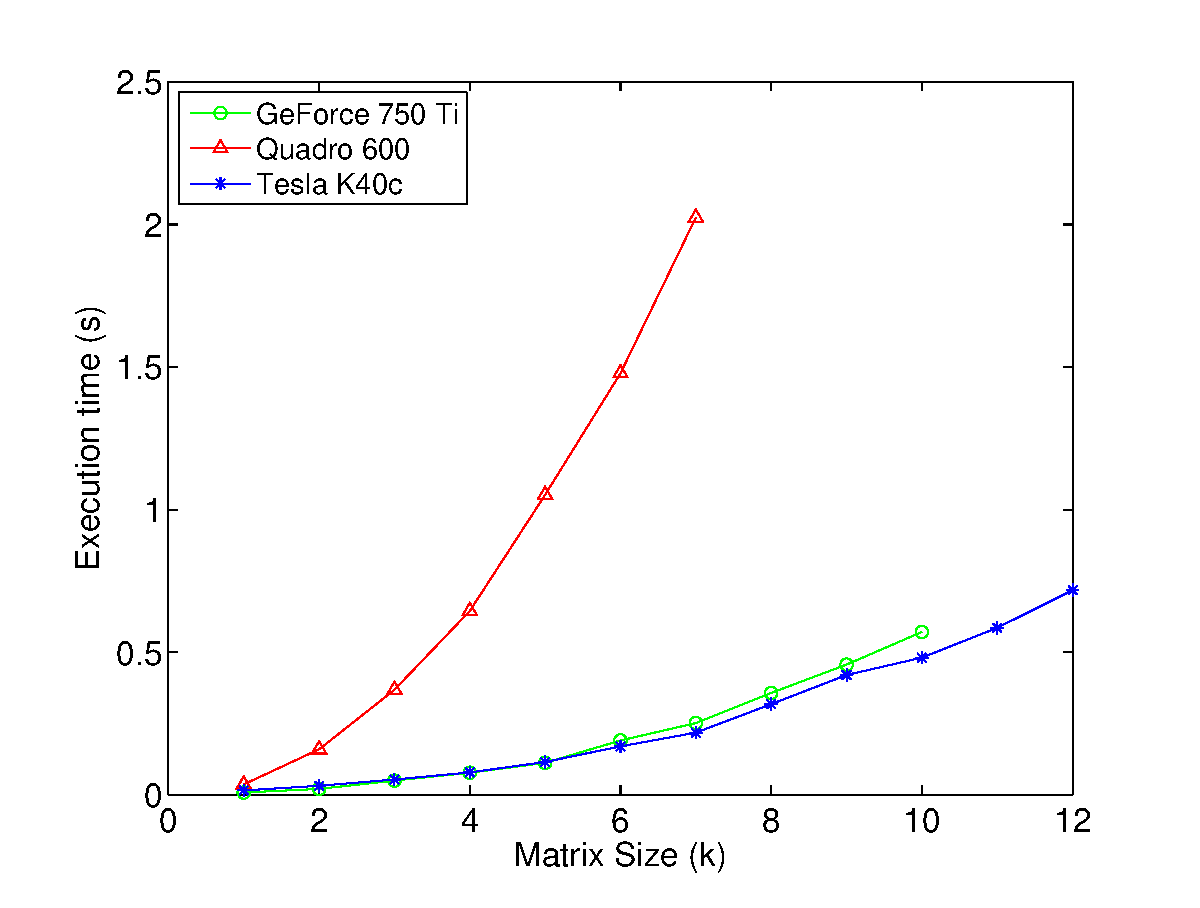
\includegraphics[width=0.3\textwidth,height=1in]{svd_vec_gpus}
    \label{fig:svd_vec}
  }
  \subfigure[Profiling Data]
  {
    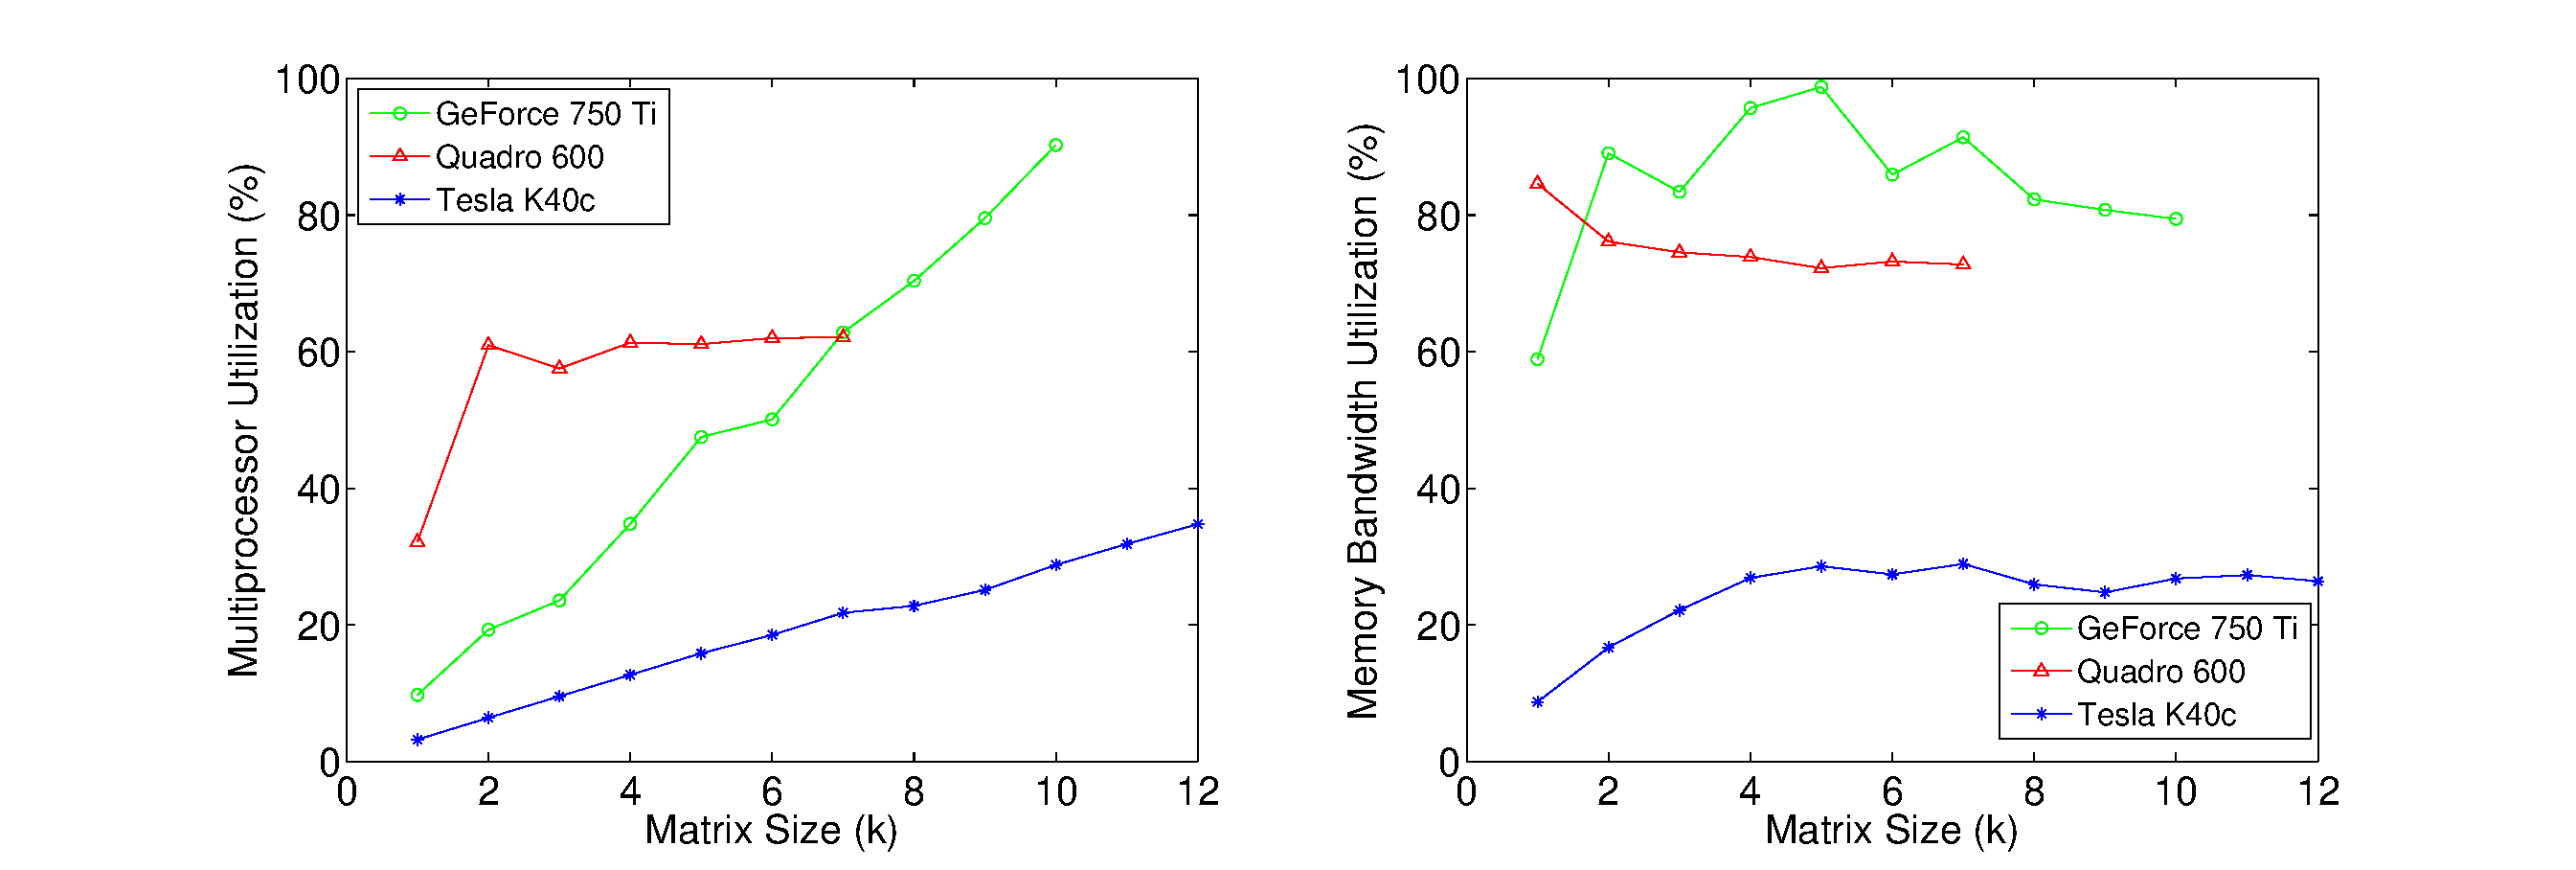
\includegraphics[width=0.6\textwidth,height=1in]{svd_vec_gpus_prof}
    \label{fig:svd_vec_prof}
  }
\vspace{-0.1in}
  \caption{Singular Vector Kernel on Different GPUs}
  \label{fig:svdvec}
\vspace{-0.3in}
\end{figure}

Figure \ref{fig:svd_vec_prof} shows thread and memory bandwidth utilizations of singular vector design on different GPUs. 
We can see from the figure that Quadro and GeForce reach a high memory utilization (80\%-99\%), while the memory utilization of Tesla is around 30\%. 
We also observe that when the matrix size is larger than 2K, the thread utilization keeps stable on Quadro. 
This is because the ratio of stall caused by memory is 70\%, implying that there are a lot of threads waiting on data transfer.
\fi 

\subsection{Huge Size Result}
Table \ref{tab:hugeResultTesla} shows the performance of huge size matrix with double-precision floating-point numbers on a single Tesla and two Tesla GPUs on a server. For two Telsa GPUs, we compared static workload allocation (50\%/50\%) and dynamic allocation where each GPU is tracked constantly by the host CPU and assigned new workload as soon as it finishes the current kernel. 
When matrix size reaches 1 million by 1 million our BT algorithm reaches the results in 54801 seconds with a single Telsa, and 35607 seconds with two Telsa GPUs. This is a 1.54X speedup.
\begin{table}[h]
\vspace{-0.3in}
\caption{Performance of Huge Size Matrix with double floating-point on Tesla}
\vspace{-0.1in}
\centering
\begin{tabular}{|c|c|c|c|}
\hline
Matrix Size &  Tesla  & Static & Dynamic \\ \hline
% 10K*10K    &   1.5s  &  1.9s / 1.2s &  0.9s / 2.5s \\ \hline
% 20K*20K    &   7.9s  &  7.4s / 5.7s &  3.1s / 10s \\ \hline
% 30K*30K    &    25s  &   17s /  14s &  12s  / 19s \\ \hline
% 40K*40K    &    38s  &   27s /  24s &  26s / 26s \\ \hline
 50K*50K    &    71s  &   50s /  45s &  44s / 44s \\ \hline
% 80K*80K    &   180s  &  121s / 103s &  111s / 116s \\ \hline
 100K*100K  &   341s  &  217s / 189s &  210s / 202s \\ \hline
% 120K*120K  &   524s  &  326s / 286s &  311s / 311s \\ \hline
 150K*150K  &   864s  &  524s / 467s &  498s / 507s \\ \hline
% 180K*180K  &   966s  & 1207s / 532s &  602s / 607s \\ \hline
 200K*200K  &  1407s  &  955s / 827s &  849s / 858s \\ \hline
% 250K*250K  &  1949s  & 1286s / 1118s & 1199s / 1204s\\ \hline
 300K*300K  &  3490s  & 2234s / 1906s & 2123s / 2110s\\ \hline
 400K*400K  &  6559s  & 4110s / 3709s & 3853s / 3871s\\ \hline
 500K*500K  & 12282s  & 7371s / 6916s  & 7148s / 7129s\\ \hline
 800K*800K  & 40311s  & 22454s / 21627s &  22046s / 22026s   \\ \hline
 1000K*1000K & 54801s  & 36119s / 35071s   &  35587s / 35607s \\ \hline
\end{tabular}
\label{tab:hugeResultTesla}
\vspace{-0.2in}
\end{table}

\subsection{Profiling Analysis of GPU Kernels}

\subsubsection{Comparison of Two Different Singular Value Designs}
We compare the execution time on two different singular value kernels:
``equal length division'' versus ``equal number division''. Each
method has two phases: (1) divide the interval into subintervals and
(2) calculate singular values in each subinterval.
%For the length division design, we selects the minimal execution time corresponding to red point curve in figure \ref{fig:length_block_num}.
%For the number division design, we selects the minimal number of blocks that is able to allocated, since the execution time does not vary much between the minimal number of blocks and the optimal nubmer of blocks.
\begin{figure}[hbpt]
\vspace{-0.3in}
\centering
  \subfigure[Comparison of Equal Length Division and Equal Number Division. ``Interval Division in EL'' is negligible.]
  {
    \includegraphics[width=0.4\textwidth]{compare_value_kernel}
    \label{fig:compare_value_kernel}
  }
  \subfigure[Memory Transactions on Singular Vector Design]
  {
    \includegraphics[width=0.4\textwidth]{transaction}
    \label{fig:transaction}
  }
\vspace{-0.1in}
%  \caption{Orthogonality of Singular Vector}
%  \label{fig:ortho}
%\vspace{-0.3in}
\end{figure}
%\begin{figure}[hbpt]
%\centering
%\includegraphics[width=0.4\textwidth]{compare_value_kernel}
%\caption{Comparison of Equal Length Division and Equal Number Division. ``Interval Division in EL'' is negligible. }
%\label{fig:compare_value_kernel}
%\vspace{-0.10in}
%\end{figure}
Figure \ref{fig:compare_value_kernel} shows the detailed execution time breakdown for each phase of both methods (``Interval Division'' time for ``equal-length division'' is negligible) on Tesla K40c.
From the figure, we can see that when the matrix size is less than 9K, the equal length division version runs a little faster than equal number division version.
However, when the matrix size exceeds 9K, the execution time of the equal length division version increases dramatically, while the execution time of equal number division version still rises linearly.
And in this case, 
%even the time to divide the interval is noticeably large, the balanced number
%of singular values in a subinterval helps improving the overall performance.
even though the time to divide the interval is noticeably
large, the balanced number of singular values in a subinterval
still yields much better performance.
Thus, the equal number division version is obviously the winner when the matrix size becomes larger than 9K.

\subsubsection{Memory Access Optimization}
We evaluate the memory optimization techniques on improving the performance
of singular vector calculation. As depicted in Figure \ref{fig:transaction},
%\begin{figure}[hbpt]
%\centering
%\includegraphics[width=0.4\textwidth]{transaction}
%\caption{Memory Transactions on Singular Vector Design}
%\label{fig:transaction}
%\vspace{-0.15in}
%\end{figure}
in the baseline design,
Global memory Load Transactions (GLT) are about twice of the Global memory Store Transactions (GST) on the global memory.
As there are 50\% of global memory transfers are read-after-write, we improve the memory access performance by copying these values into the local memory and shared memory of the GPU. As a result, the GLT are reduced by 50\% compared to the baseline, while the GST remains the same, labeled as ``Read/Write Optimization'' in Figure \ref{fig:transaction}. The speedup on singular vector calculation reaches to 1.2X compared to the baseline.
Changing the matrix arrangement from row-major to column-major in the global memory 
reduces GLT and GST by 50\% and 25\%, respectively, compared to ``Read/Write optimization''. 
This is because column-major matrix have coalesced global memory accesses, which saves hundreds of transactions per thread. The speedup rises up to 4.5X compared to the baseline.

\subsection{Accuracy Analysis}
\subsection{Tolerance in Bisection Algorithm}
Since the bisection algorithm is an approximate algorithm to calculate the singular values, we should test the effect of different error tolerance.
The error tolerance $err$ means that the error between the singular values of our algorithm and the actual singular values are less than $err$.
It determines the accuracy of singular value and therefore the orthogonality of singular vectors.
As we know, the more accuracy of singular values are, the more execution time should be spent.
However, it is important to know the incremental execution time to determine which error tolerance is suitable for different applications.
We test our algorithm on different error tolerance.
The error tolerance is between $10^{-5}$ to $10^{-16}$ with tenfolder decreasing.

%\textbf{I'm still thinking how to draw this figure.}
\begin{figure}[hbpt]
\centering
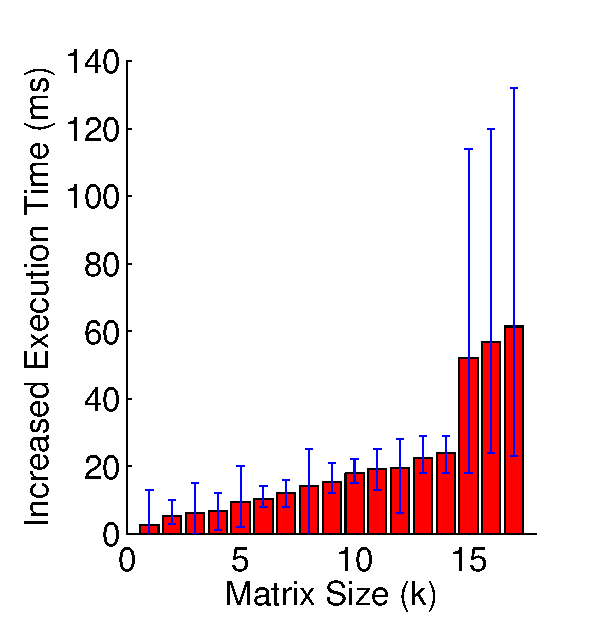
\includegraphics[width=0.5\textwidth]{tolerance}
\caption{Average Extra Execution Time When the accuracy increase Performance Comparision}
\label{fig:tolerance}
\end{figure}
Figure \ref{fig:tolerance} shows the average increased execution time when the accuracy of singular values goes up a higher level on different matrix size.
In other word, it shows the average increased execution time when the error tolerance becomes smaller from $10^{-x}$ to $10^{-(x+1)}$.
From the figure, we can see that when matrix size is smaller than 12000, the additional execution time is only less than $20 ms$ when the error tolerance rises a level.
When the matrix size is larger than 15000, the additional execution time is a little higher about $40 ms$ per level.

\subsubsection{Orthogonality of Singular Vector}
In this section, I will show the orthogonality of singular vectors. 
The multiplication of singular vectors is shown in \ref{fig:ortho_img}. The white diagonal are 1s, and the black are 0s. 
The error distribution of orthogonality is shown in \ref{fig:ortho_err}. Almost all the errors are close to 0.
\begin{figure}[hbpt]
\vspace{-0.3in}
\centering
  \subfigure[Orthogonal Error]
  {
    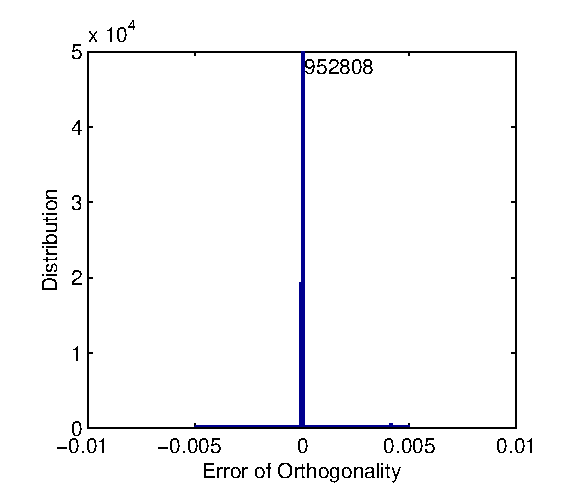
\includegraphics[width=0.4\textwidth]{ortho_err}
    \label{fig:ortho_err}
  }
  \subfigure[Image of Singular Vector Multiplication]
  {
    \includegraphics[width=0.4\textwidth]{orthogonal}
    \label{fig:ortho_img}
  }
\vspace{-0.1in}
  \caption{Orthogonality of Singular Vector}
  \label{fig:ortho}
\vspace{-0.3in}
\end{figure}
